\documentclass[11pt]{article}
\usepackage{classTools}
\usepackage[normalem]{ulem}
\sloppy

\begin{document}

% To include a problems set header, use the psHeader command
\psHeader{8}{Wed Nov. 29, 2023 (11:59pm)}


\textbf{Your name: Cory Zimmerman}

\textbf{Collaborators:} \\
I'm listing ChatGPT as a collaborator, but "collaboration" was within the fair use policy. The most helpful thing ChatGPT did was generate test data for me to try out my proof hypotheses (ex. generating interesting CNFs to test my reduction for question one on).

\textbf{No. of late days used on previous psets: 0}

\textbf{No. of late days used after including this pset: 0}

\textbf{Please fill out feedback form:} \href{https://forms.gle/K4Z1b1EhsT8dRY2T6}{https://forms.gle/K4Z1b1EhsT8dRY2T6}.

\vspace{1em}

\noindent The purpose of this problem set is to to reinforce the definitions of $\Psearch$, $\EXPsearch$, $\NPsearch$, and $\NPsearch$-completeness and practice $\NP$-completeness proofs. 

\begin{enumerate}
    \item (Positive Monotone SAT)
    A boolean formula is {\em positive monotone} if there are no negations in it.  Restricting SAT to positive monotone formulas makes it a trivial problem: setting all variables to 1 is always a satisfying assignment.
    
    However, the following variant of Positive Monotone SAT is more interesting:
    
        \compprob{$k$-False PositiveMonotoneSAT()}
        {A positive monotone CNF formula $\varphi(x_0,\ldots,x_{n-1})$ and a number $k\in \N$}
        {A satisfying assignment $\alpha\in\zo^n$ in which at least $k$ variables are set to 0 (if one exists)}
    
    \begin{enumerate}
        \item Prove that $k$-False PositiveMonotoneSAT is $\NPsearch$-complete, even when $k=n/2$.  (Hint: reduce from SAT, replacing negated variables with new ones and adding additional clauses.)
        \begin{quote}
            \color{purple}
            \textit{(1) k-False PositiveMonotoneSat is in $\NP_{search}$}: \\

            Polynomial length output: Given a boolean formula with $n$ variables, k-False PositiveMonotoneSat will return an assignment of those variables to either true or false. The output of $n$ assignments is thus of the same order of magnitude as the inputs and is of polynomial size. Reaching the same point from a different angle, k-False PositiveMonotoneSat is a variant of SAT. The output of SAT is known to be of polynomial length, so k-False PositiveMonotoneSat output should also have polynomial length.  \\

            Polynomial time verification: Given a possible assignment, run the same verifier from SAT on the assignment from k-False PositiveMonotoneSat against the given formula. If the assignment is correct and the number of variables set to zero is greater than or equal to $k$, then the output is correct. Else, it's incorrect. The verifier for SAT is known to take polynomial time, and the number of variables set to zero can be counted in $O(n)$ steps, so it must be the case the k-False PositiveMonotoneSAT output can be verified in polynomial time. \\

            \textit{(2) k-False PositiveMonotoneSAT is $\NP_{search}$-hard}: \\

            I'll prove hardness by reducing SAT to k-False PositiveMonotoneSAT in polynomial time: \\

            Let $\varphi(x_0, \dots, x_{n - 1})$ be any arbitrarily chosen boolean formula with $n$ total variables. This must be transformed into a formula with no negations. So, for each variable $x_0, \dots, x_{n - 1}$, let there be some $\alpha_0, \dots, \alpha_{n - 1}$ such that $\alpha_i = \neg x_i$ for all $0 \leq i < n$. \\

            Transform $\varphi(x_0, \dots, x_{n - 1})$ into $\varphi(x_0, \alpha_0, \dots, x_{n - 1}, \alpha_{n - 1})$ by replacing every instance of a negated variable $\neg x_i$ with $\alpha_i$. These replacements will require as many steps as there are terms in the formula. \\

            Then, prepend $n$ clauses to the CNF of the form $(x_i \lor \alpha_i)$ for each $0 \leq i < n$. This will require some polynomial number of steps for each $n$ new clause, with specific runtime dictated by the representation of the CNF. \\

            Next, make a single oracle call to k-False PositiveMonotoneSAT. By this point, the boolean formula has $n' = 2n$ variables. In the oracle call, set $k = \frac{n'}{2} = n$. If the output is $\bot$, return $\bot$. Else, collect the output assignment. Everywhere $\alpha_i$ is true, mark $x_i$ as false. This process requires $n'$ steps to consider every $x_i$ and $\alpha_i$ that's assigned. This assignment should then be returned. \\

            Assuming the k-False PositiveMonotoneSAT oracle is correct, the correctness of this reduction depends on the correctness of my encoding of the inputs. Because of the $\alpha$ substitutions, k-False PositiveMonotoneSAT will receive a boolean formula representing the input formula without any negations. By prepending $n$ clauses to the beginning of the formula of the form $(x_i \lor \alpha_i)$, every boolean state present in or implied by the formula is explicitly defined. Because $k = \frac{n'}{2} = n$ of these variables must be false and every clause only contains two variables, one variable in every clause must be false. Thus, every state is exclusively true or false in the output assignment. Because of this, the reduction correctly encodes the input to SAT. The output decoding simply reverses the $\alpha$ encoding, preserving correctness. So, the reduction must be correct. \\

            The steps in this reduction involve single-pass traversals of the input variables and the length of the CNF. Because all of these steps require polynomial time, my algorithm reduces to k-False PositiveMonotoneSAT in polynomial time. This demonstrates that k-False PositiveMonotoneSAT is $\NP_{search}$-hard. \\

            \textit{Conclusion}: \\ 
            Because k-False PositiveMonotoneSAT is in $\NP_{search}$ and SAT can be reduced to k-False PositiveMonotoneSAT in polynomial time, it must be the case that k-False PositiveMonotoneSAT is $\NP_{search}$-complete. \\

            \textit{Example}: \\
            The example below shows how an input boolean formula is tranformed into input for k-False PositiveMonotoneSAT by introducing $\alpha$ variables and adding additional clauses. Solved output is then parsed and returned as a satisfying assignment that solves SAT.  
            \noindent
            \begin{figure}[ht]
                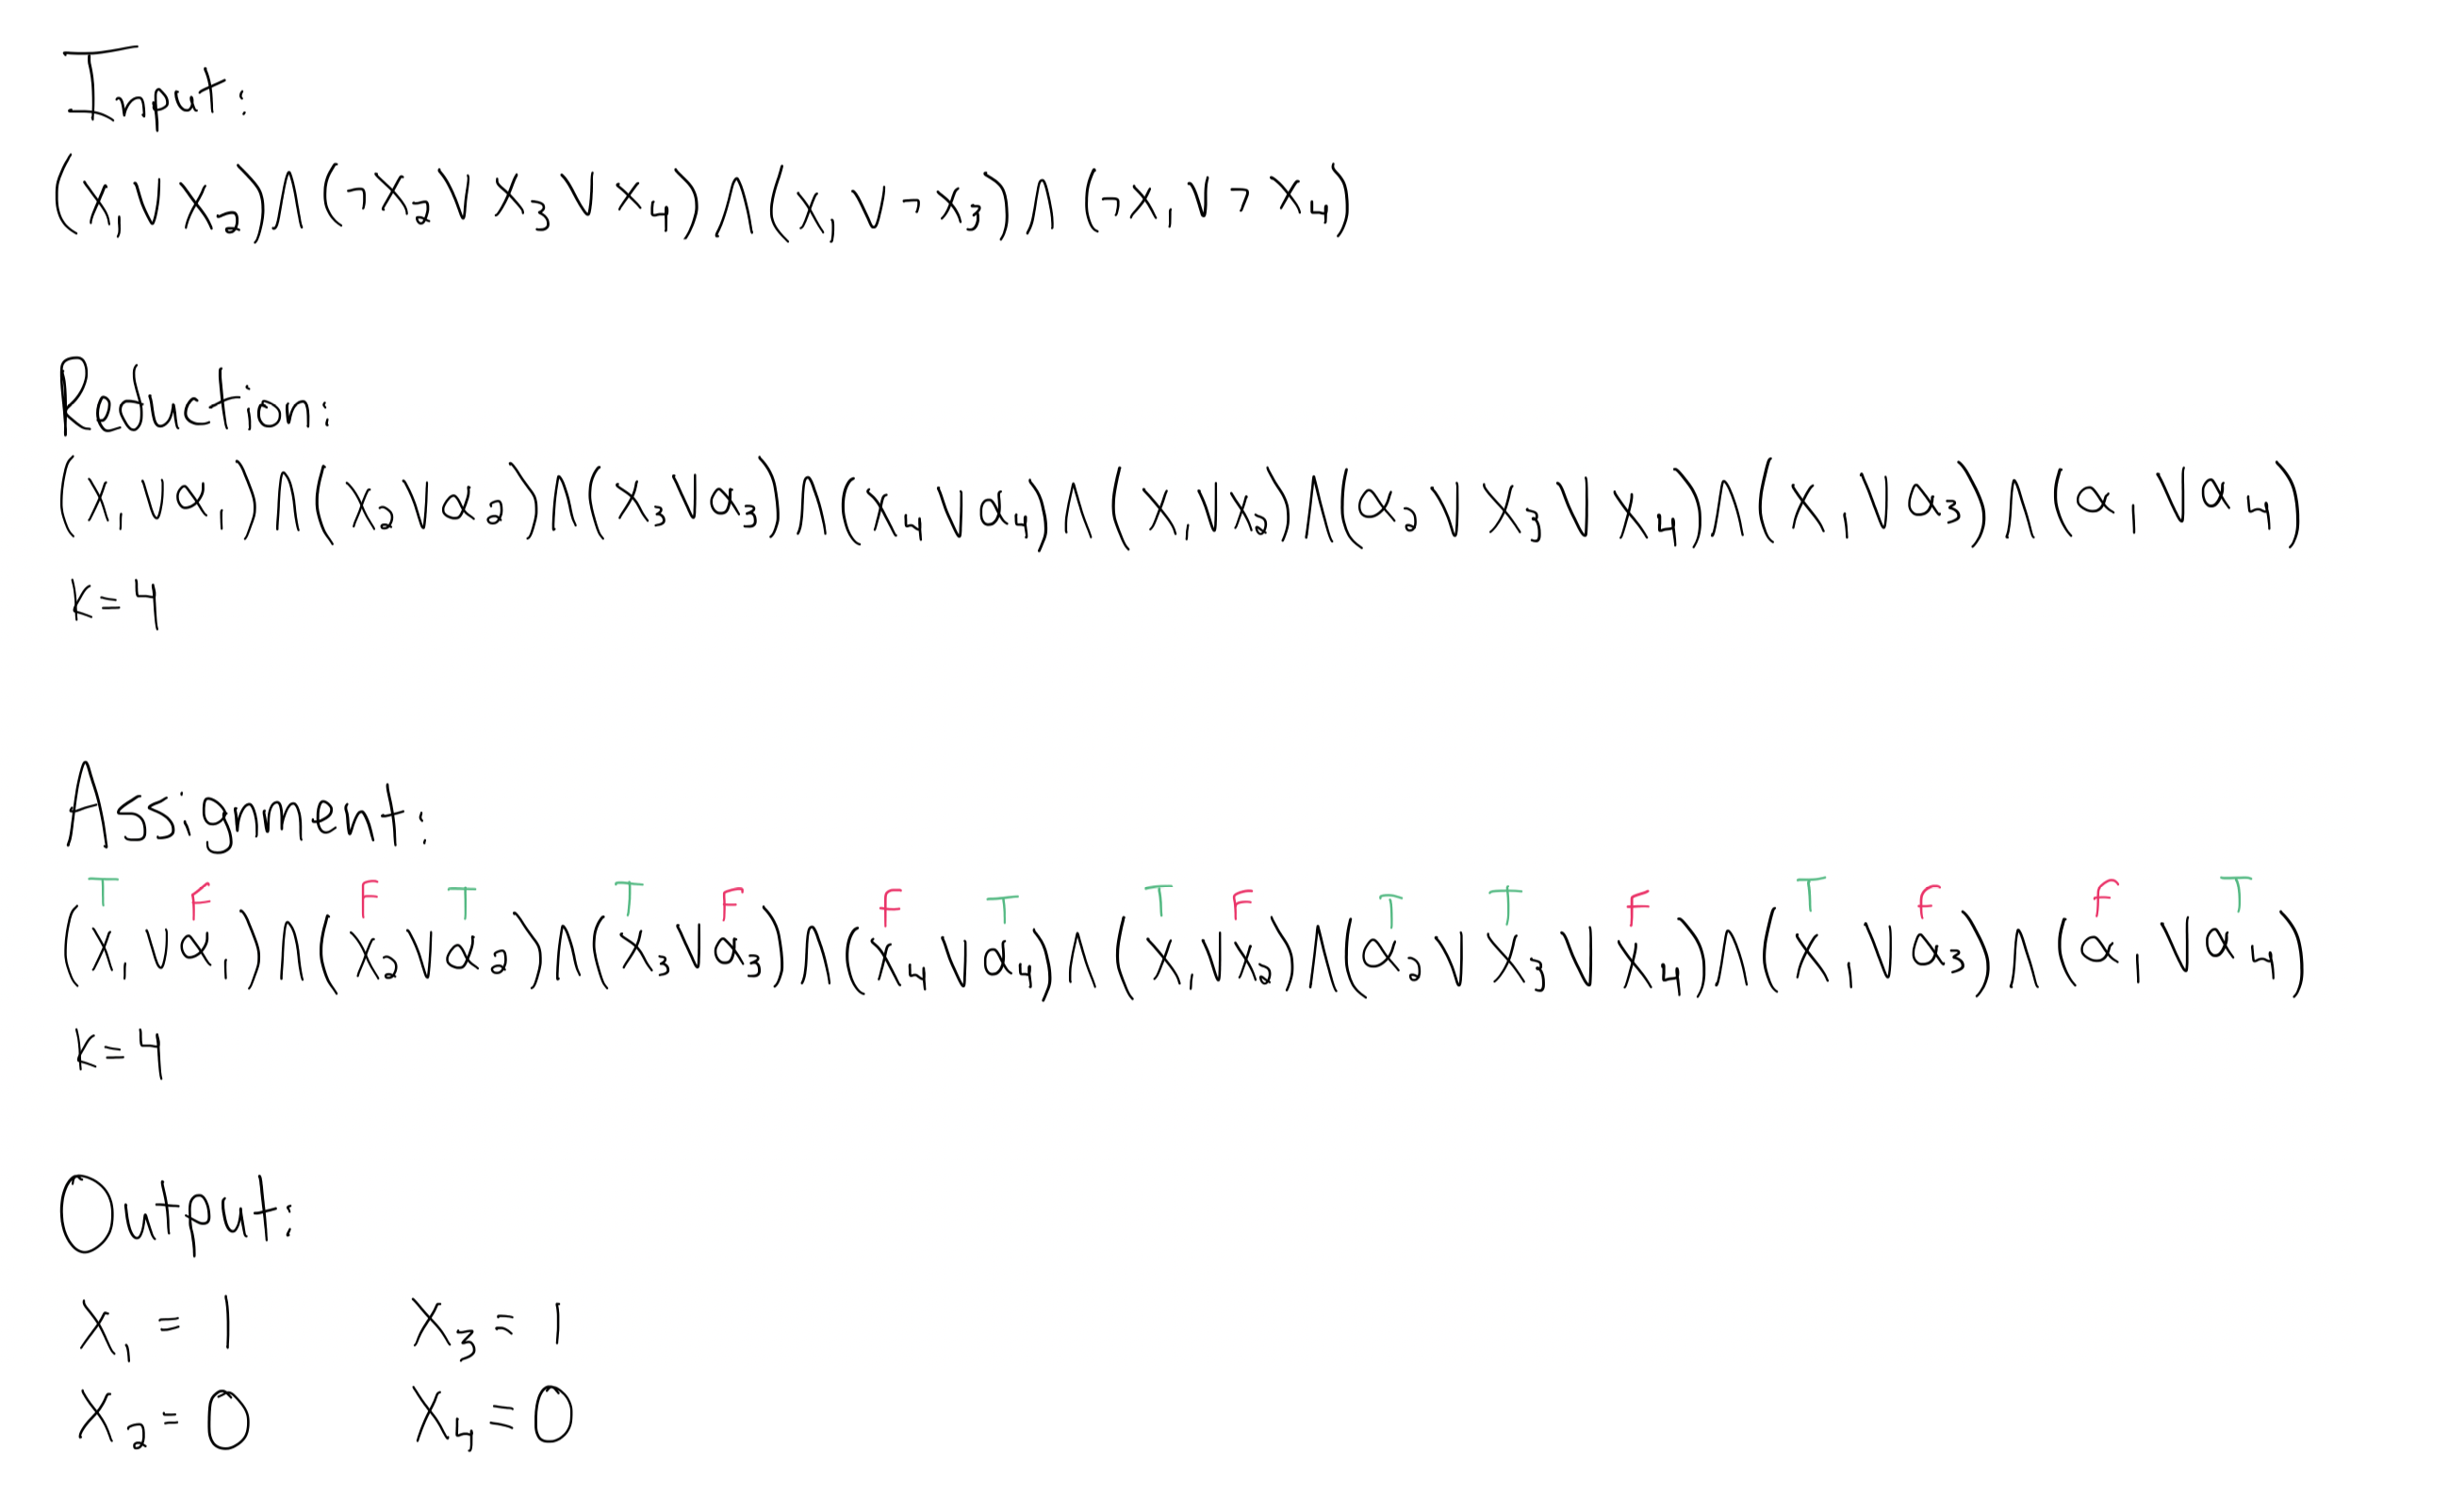
\includegraphics[scale=0.4]{kfpms reduction example.png} 
            \end{figure}

        \end{quote}
        
        \item Prove that if we fix $k=3$, then $k$-False PositiveMonotoneSAT is in $\Psearch$. (Hint: show that it suffices to consider assignments in which exactly 3 variables are set to 0.)
        \begin{quote}
            \color{purple}
            \textit{Lemma}: If a satisfying assignment with $3 \leq j$ variables set to zero exists, then a satisfying assignment with exactly three variables set to zero exists. Prove this inductively: \\

            Base case: When the satisfying assignment already contains exactly three zeroes, the claim is trivially true. \\

            Inductive hypothesis: Assume that if a satisfying assignment with exactly $j$ variables set to zero exists where $3 \leq j$, then a satisfying assignment with exactly three variables set to zero exists. \\

            Inductive step: Consider a satisfying assignment with exactly $j + 1$ variables set to zero. Because the assignment satisfies a CNF, every clause in the CNF already resolves true. Choose any arbitrary zero variable and flip it to one. Every clause in the CNF still resolves true, and there are now $j$ variables set to zero. By the inductive hypothesis, there must exist a satisfying assignment to this CNF with exactly three variables set to zero. \\

            By induction, it must then be true that if a satisfying assignment with $3 \leq j$ variables set to zero exists, then a satisfying assignment with exactly three variables set to zero exists. \\

            \textit{Proof}: \\

            Assert the following from the lemma above: if a given formula has a satisfying assignment with more than three variables set to zero, it also has a satisfying assignment with exactly three variables set to zero. So, I'll prove that such a solution with exactly three variables set to zero can be found in polynomial time: \\
            
            k-False PositiveMonotoneSAT can be solved in polynomial time when a satisfying assignment of exactly three "zero values" exists by running the following algorithm: \\

            \begin{itemize}
                \item For each $i$ from $0$ to $n - 3$:
                \begin{itemize}
                    \item For each $j$ from $i + 1$ to $n - 2$:
                    \begin{itemize}
                        \item For each $k$ from $j + 1$ to $n - 1$:
                        \begin{itemize}
                            \item Check if the formula is satisfied when $x_i$, $x_j$, and $x_k$ are zero and all other values are one. If so, return that assignment. Else, continue checking.
                        \end{itemize}
                    \end{itemize}
                \end{itemize}
                \item If no assignment was found after checking all combinations, return $\bot$.
            \end{itemize}

            This algorithm considers every possible combination of exactly three variables within the boolean formula. If a satisfying assignment exists in which these three variables are false, such an assignment will be returned. The three loops take $O(n^3)$ time where $n$ is the number of variables. The SAT verifier takes some polynomial time $O(m^c)$ where $c$ is a constant and $m$ is the number of terms. So, this algorithm takes polynomial time $O(n^3 \cdot m^c)$ to find an assignment with exactly three variables set to zero if one exists. Because this encompasses every possible formula that can be solved by PositiveMonotoneSAT with $k = 3$, it must be the case that k-False PositiveMonotoneSAT is in $P_{search}$. \\
            
        \end{quote}

        
        \item (optional\footnote{This problem is meant to be done based on your enjoyment/interest and only if you have time. It won't make a difference between N, L, R-, and R grades, and course staff will deprioritize questions about this problem at office hours and on Ed.}) Show that $k$-False PositiveMonotone 2-SAT is $\NPsearch$-complete.  (Hint: reduce from Independent Set.)
    \end{enumerate}


    \item (Reductions and complexity classes)  
    \begin{enumerate}
        \item Prove that if a problem $\Pi$ is in $\Psearch$, then $\Pi\leq_p \Gamma$ for all computational problems $\Gamma$.

        \begin{quote}
            \color{purple}
            Because $\Pi$ is in $\Psearch$, it can be solved in polynomial time. Assuming we're defining a Turing reduction, we have the option to call an oracle for $\Gamma$ an arbitrary number of times. So, consider this reduction for any problem $\Pi$ in $\Psearch$ that reduces to $\Gamma$ but makes no oracle calls: \\

            Given inputs and an algorithm for $\Pi$, run the algorithm on the inputs to generate the output. Return that output. \\

            Because $\Pi$ is in $\Psearch$, it runs in polynomial time. Because the algorithm solves $\Pi$, the output is correct. This reduction technically reduces to $\Gamma$ in polynomial time while making exactly zero oracle calls. Because $\Gamma$ can be any problem and $\Pi$ will still be "reduced" in polynomial time, it must be the case that $\Pi \leq_p \Gamma$ for any computational problem $\Gamma$ when $\Pi$ is in $\Psearch$. \\
        \end{quote}

        
        \item Show that if $\NPsearch\subseteq \Psearch$, then all problems in $\NPsearch$ are $\NPsearch$-complete.  (The converse of this statement was proved in section, so it is actually an iff.)  
        \begin{quote}
            \color{purple}
            Assume $\NPsearch$ is a subset of $\Psearch$ and prove the claim directly by examining any arbitrarily chosen problem $\Pi$ from $\NPsearch$. \\

            \textit{$\Pi$ is in $\NPsearch$}: \\
            This is true because $\Pi$ was chosen from $\NPsearch$. \\

            \textit{$\Pi$ is $\NPsearch$-hard}: \\
            This requires demonstrating that every problem in $\NPsearch$ reduces in polynomial time to $\Pi$. Let $\Gamma$ be any arbitrarily chosen problem from $\NPsearch$. By the initial assumption that $\NPsearch$ is a subset of $\Psearch$, it must be the case that $\Gamma$ is in $\Psearch$. By the proof for part $(a)$, it must be true that $\Gamma$ reduces in polynomial time to any computational problem. Because $\Pi$ is a computational problem, it must be true that $\Gamma$ reduces to $\Pi$ in polynomial time. Because $\Gamma$ can be any problem from $\NPsearch$, it must be the case that all problems in $\NPsearch$ reduce in polynomial time to $\Pi$. This proves that $\Pi$ is $\NP_{hard}$. \\

            \textit{Conclusion}: \\
            Because $\Pi$ is in $\NPsearch$ and is $\NP_{hard}$, it must be the case that $\Pi$ is $\NPsearch$-complete. Because $\Pi$ can be any arbitrarily chosen problem from $\NPsearch$, it must be the case that, if $\NPsearch$ is a subset of $\Psearch$, then all problems in $\NPsearch$ are $\NPsearch$-complete. \\ 
            
        \end{quote}
        
        \item  Prove that if 
$\Pi\leq_p \Gamma$ and $\Gamma\in \EXPsearch$, then $\Pi\in \EXPsearch$. (In other words, $\EXPsearch$ is closed under polynomial-time reductions.) 

\begin{quote}
    \color{purple}
    Let $\Pi$ be any computational problem and let $\Gamma$ be any problem in $\EXPsearch$ such that $\Pi$ reduces to $\Gamma$ in polynomial time. \\

    Because such a reduction exists, let $\pi$ represent the polynomial time algorithm implementing the reduction such that the runtime of $\pi$ is $O(n^{c_1})$ where $c_1$ is a constant. Let $\gamma$ represent the most efficient algorithm solving $\Gamma$ such that the runtime of $\gamma$ is $O(2^{n^{c_2}})$ where $c_2$ is a constant. \\

    For every place in $\pi$ that the oracle for $\Gamma$ is called, replace the oracle call with the actual algorithm $\gamma$. Doing so leaves an augmented algorithm $\pi'$ that solves $\Pi$ without any reduction. Because the polynomial time reduction can call the oracle at most a polynomial number of times, the runtime of $\pi'$ is bounded by $O(n^{c_1} \cdot 2^{n^{c_2}})$, which is at most exponential. This demonstrates the existence of an algorithm solving $\Pi$ in at-most exponential time. So, if $\Pi$ reduces in polynomial time to $\Gamma$ and $\Gamma$ is in $\EXPsearch$, then $\Pi$ is in $\EXPsearch$. \\
    
    Note additionally that $\pi'$ may actually run in polynomial time, but, because $\Psearch$ is a subset of $\EXPsearch$, it's still the case that $\Pi$ is in $\EXPsearch$, even if a more specific classification could also be provided. 
\end{quote}
    \end{enumerate}

\newpage

\item (Variant of VectorSubsetSum)  
In the Sender--Receiver Exercise on November 16, you will see that the following problem is $\NPsearch$-complete.

\compprob{VectorSubsetSum()}
{Vectors $\vec{v}_0,\vec{v}_1,\ldots,\vec{v}_{n-1}\in \zo^d$, $\vec{t}\in \N^d$}
{A subset $S\subseteq [n]$ such that $\sum_{i\in S}\vec{v}_i = \vec{t}$, if such a subset $S$ exists.}

We will use the notation $\vec{v}[j]$ to denote the $j$'th entry of vector $\vec{v}$, so the condition 
$\sum_{i\in S}\vec{v}_i = \vec{t}$ means that for every $j=0,1,\ldots,d-1$, we have $\sum_{i\in S}\vec{v}_i[j] = \vec{t}[j]$.

Assuming that result, prove that the following variant is also $\NPsearch$-complete.
    
    \compprob{VectorSubsetSumVariant()}
{Vectors $\vec{v}_0,\vec{v}_1,\ldots,\vec{v}_{n-1}\in \N^d$, $t_0\in \N$}
{A subset $S\subseteq [n]$ such that $\sum_{i\in S}\vec{v}_i = (t_0,t_0,\ldots,t_0)$, if such a subset $S$ exists.}

    The two differences from the VectorSubsetSum problem is that the vectors are no longer restricted to have $\zo$ entries, but now all entries of the target vector are required to be equal. (Hint: reduce from the standard VectorSubsetSum problem.  Add an additional vector and an additional coordinate.)

    \end{enumerate}

    \begin{quote}
        \color{purple}
        I'll prove that VectorSubsetSumVariant (VSSV) is $\NPsearch$-complete directly by first proving that it's in $\NPsearch$ and then by demonstrating that every problem in $\NPsearch$ reduces to VSSV in polynomial time. \\

        \textit{VSSV is in $\NPsearch$}: \\
        Proving that VSSV is in $\NPsearch$ requires demonstrating that all solutions are of polynomial length and solutions are verifiable in polynomial time. \\
        
        Solution length: Consider input of bit size $n$. In the case that every vector is chosen by VSSV, the greatest possible output is every vector, which is of size $n$. Because of this, output is at most a polynomial size greater than input. \\

        Verification time: Given any set of vectors, their validity as a solution to VSSV can be verified by adding the values in every column of every vector and checking if every column sums to the target value. This requires iterating through at most the input size once, which takes time no more than polynomially greater than the input size. \\

        Because these two conditions are satisfied, it must be the case that VSSV is in $\NPsearch$. \\

        \textit{VSSV is $\NPsearch$-hard}: \\
        By the SRE, assert that VectorSubsetSum is $\NPsearch$-complete. Because of this, it must be true that every problem in $\NPsearch$ reduces in polynomial time to VectorSubsetSum. By proving that VectorSubsetSum reduces to VSSV in polynomial time, I will thus prove that every problem in $\NPsearch$ reduces to VSSV in polynomial time. \\

        Consider the following algorithm to reduce VectorSubsetSum to VSSV: 

    \begin{enumerate}
        \item Assign a variable $t_{max}$ to be the maximum value among all entries in the input vector $\Vec{t}$.
        \item (Optional, for clarity) Rename the input vector $\Vec{t}$ to $\Vec{t}_{input}$.
        \item Create a new vector $\Vec{v}_{balance}$ and add it to $V$. 
        \item For each index $i$ of the vector length, set $\Vec{v}_{balance}[i] = t_{max} - \Vec{t}_{input}[i]$. 
        \item Add a new column to every input vector. For $\Vec{v}_{balance}$, set that column to $t_{max}$. For every other vector in $V$, set that column to $0$.
        \item Call VectorSubsetSumVariant on the modified vectors $\Vec{v_0}, \Vec{v_1}, \dots, \Vec{v}_{n - 1}, \Vec{v}_{balance}$ with $t_0$ set to $t_{max}$.
        \item If VSSV output is $\bot$, return $\bot$. Else, remove $\Vec{v}_{balance}$ from the output, and remove the added column from every remaining vector such that every vector has the same columns it started with. Return those vectors.
    \end{enumerate}

    Correctness: \\
    Begin by considering the column the reduction adds to every input vector. Because the output must add up to $t_{max}$ in every column and $\Vec{v}_{balance}$ is the only vector that can satisfy this, $\Vec{v}_{balance}$ is guaranteed to be in any non-$\bot$ output. \\

    After $\Vec{v}_{balance}$ is selected, VSSV now needs to select vectors such that the sum of the columns of those vectors adds up to $t_{max} - \Vec{v}_{balance}[i]$ for every vector index $i$. Because of step four in the algorithm, the value $t_{max} - \Vec{v}_{balance}[i]$ is guaranteed to be $\Vec{t}_{input}[i]$. Thus, after $\Vec{v}_{balance}$ is selected, VSSV proceeds to select vectors based on the input columns such that they sum to the input target. Through this process, VSSV selects $\Vec{v}_{balance}$ and a correct solution to VectorSubsetSum if one exists and returns it. My reduction takes out $\Vec{v}_{balance}$ and removes the extra column to produce exactly the solution to VectorSubsetSum if one exists. Because of this, my VSSV reduction must be correct. \\

    Runtime: \\
    If each input vector is of length $n$, then iterating through $\Vec{t}_{input}$ to find $t_{max}$ takes $O(n)$ time. Creating and assigning $\Vec{v}_{balance}$ also requires iterating vectors of length $n$, which means my reduction still requires $O(n)$ time. Instantiating a new column in $m$ total vectors requires $O(m)$ time assuming constant time vector push, and removing those columns from output requires the the same complexity. Thus, my reduction runs in polynomial time $O(n + m)$. Even if individual steps in the algorithm take more time on a given model of computation, this runtime is still guaranteed to be polynomial by the extended Church-Turing thesis. \\

    Because of this polynomial time reduction from VectorSubsetSum to VSSV, assert that every problem in $\NPsearch$ reduces to VSSV, making VSSV $\NPsearch$-hard. \\ 

    \textit{Conclusion}: \\
    Having proven that VectorSubsetSumVariant is in $\NPsearch$ and is $\NPsearch$-hard, it must be true that VectorSubsetSumVariant is $\NPsearch$-complete. \\

    \textit{Example}: \\
    Here's an example of how the input to VectorSubsetSum is transformed into input for VSSV through my reduction. The input vectors are the same as those given in the SRE example, where the entries of $v_i$ can be read left to right and $t$ represents the target vector. I changed the names in my proof, so $v_{new}$ is equivalent to $\Vec{v}_{balance}$ and $t_{new}$ is a vector of all $t_0 = t_{max}$.
    
    \noindent
    \begin{figure}[ht]
        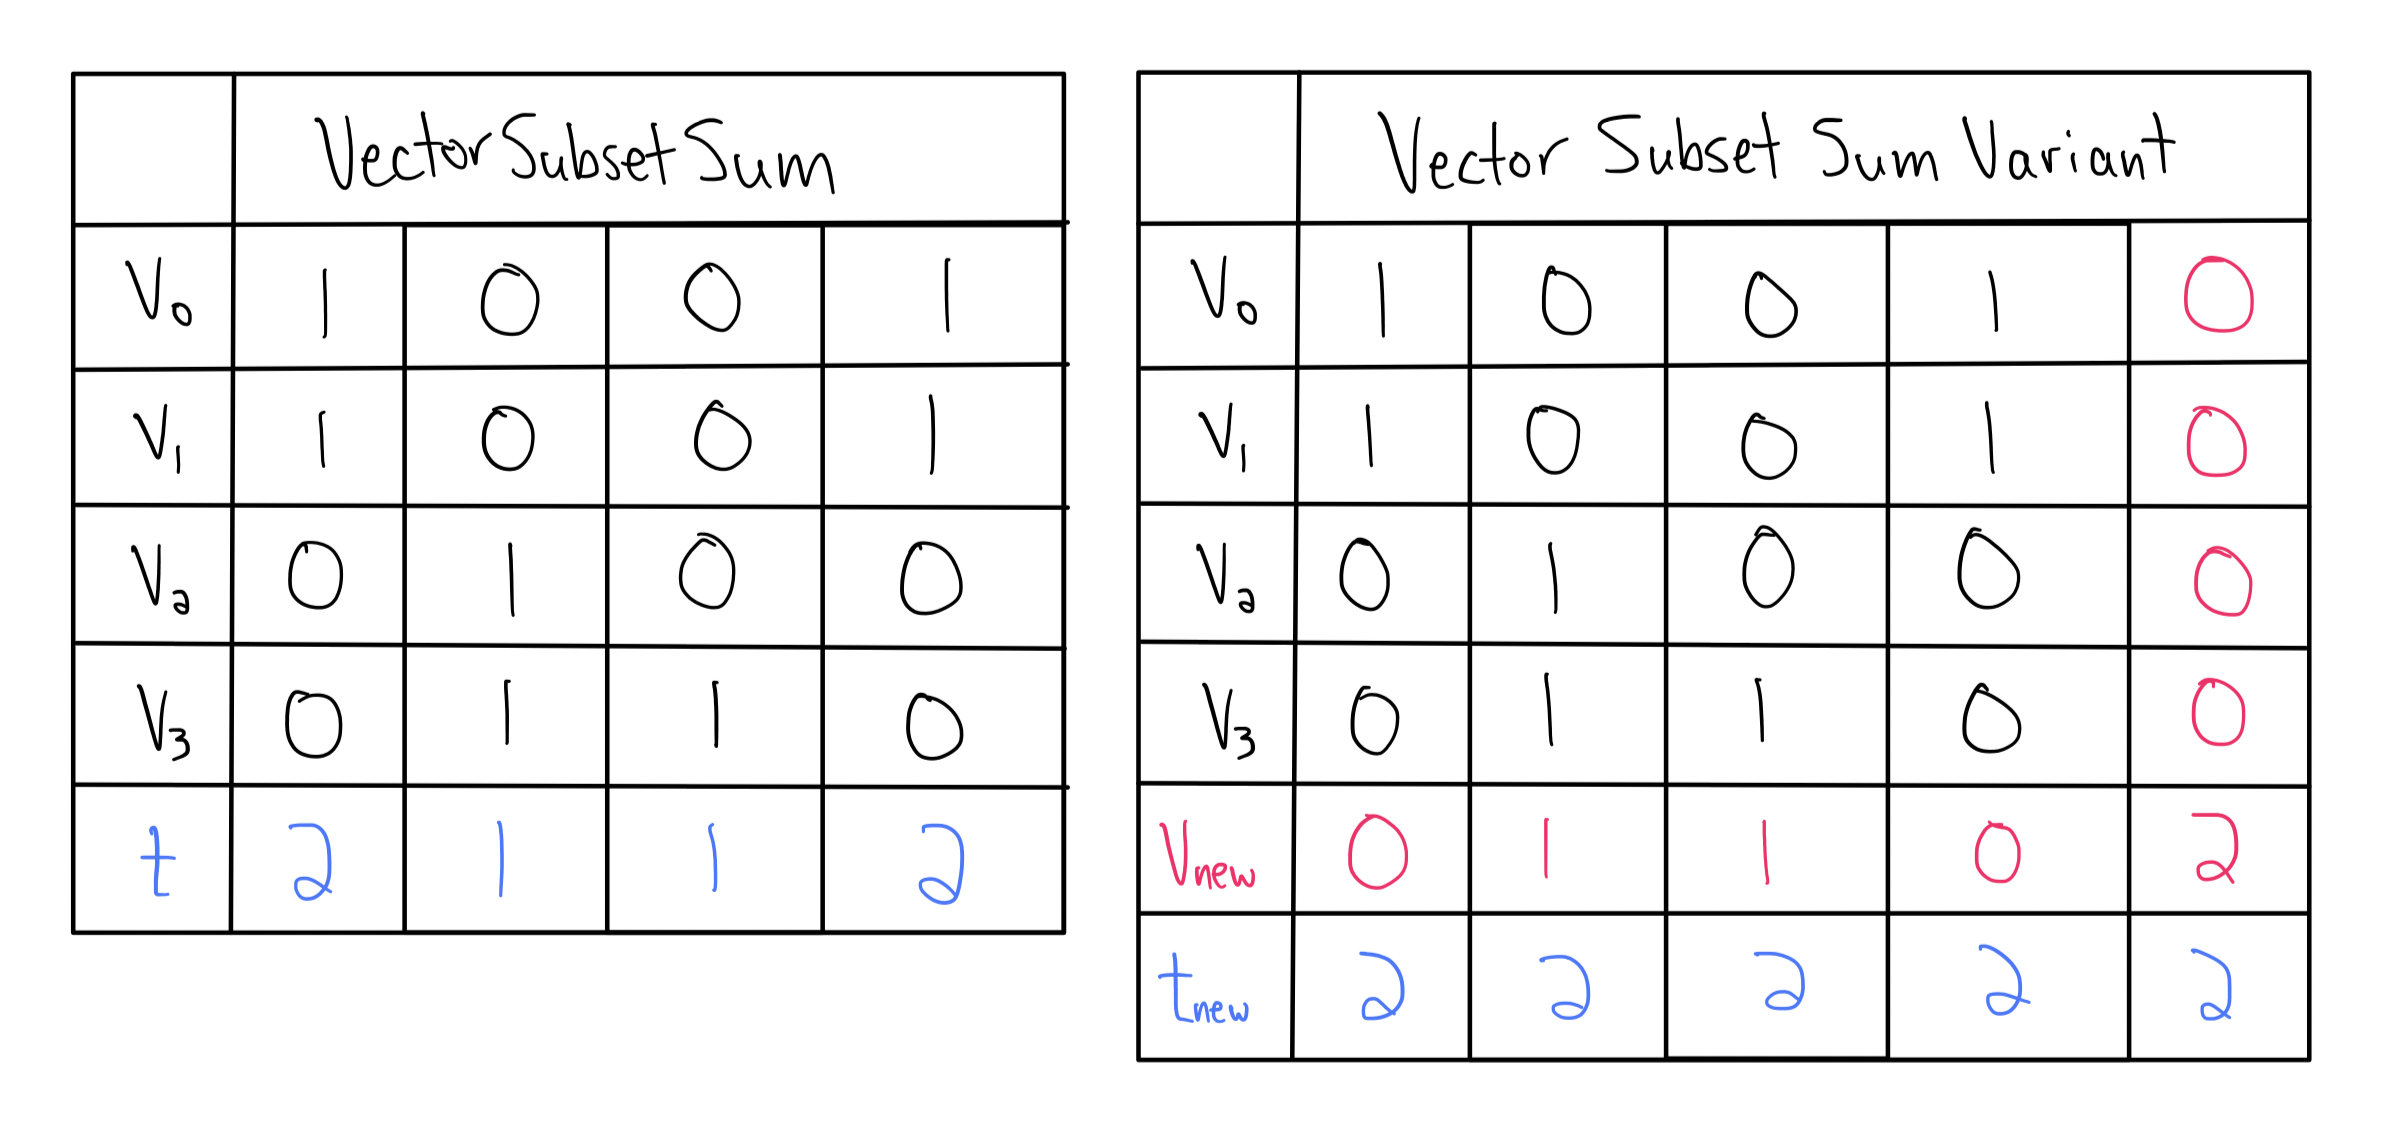
\includegraphics[scale=0.4]{vssv reduction example.png} 
    \end{figure}
    \end{quote}
    

\end{document}
